\section{Eywa Agentic Systems: Multi-Agent Composition and Orchestration}

With EywaAgent defined as a plug-and-play building block for agentic AI systems, we naturally extend this paradigm to multi-agent settings to enable more complex and heterogeneous collaborations. 
To this end, we introduce two complementary system-level abstractions. First, \textit{EywaMAS} generalizes EywaAgent to a distributed multi-agent setting, allowing multiple specialized agents to interact and collaborate. Second, \textit{EywaOrchestra} introduces a global orchestration mechanism that dynamically coordinates agents through structured planning and execution to solve complex tasks.

\subsection{EywaMAS: Plug-and-Play Composition with EywaAgent}

\begin{tcolorbox}[
  agentscope,
  float,
  floatplacement=h,
  title=\textbf{EywaMAS}
]
\begin{definition}[EywaMAS]
An \textit{EywaMAS} is defined as a multi-agent system
\begin{equation}
\mathcal{M}_{\mathrm{Eywa}} = (\mathcal{A}, \mathcal{G})
\end{equation}
where $\mathcal{A} = \{\mathcal{A}_1, \dots, \mathcal{A}_n\}$ is a set of heterogeneous agents, each of which is either an LLM agent or an EywaAgent, and $\mathcal{G}$ specifies the communication topology.
\end{definition}
\end{tcolorbox}

\begin{wrapfigure}{r}{0.30\textwidth}
  \begin{center}
  \vspace{-19pt}
    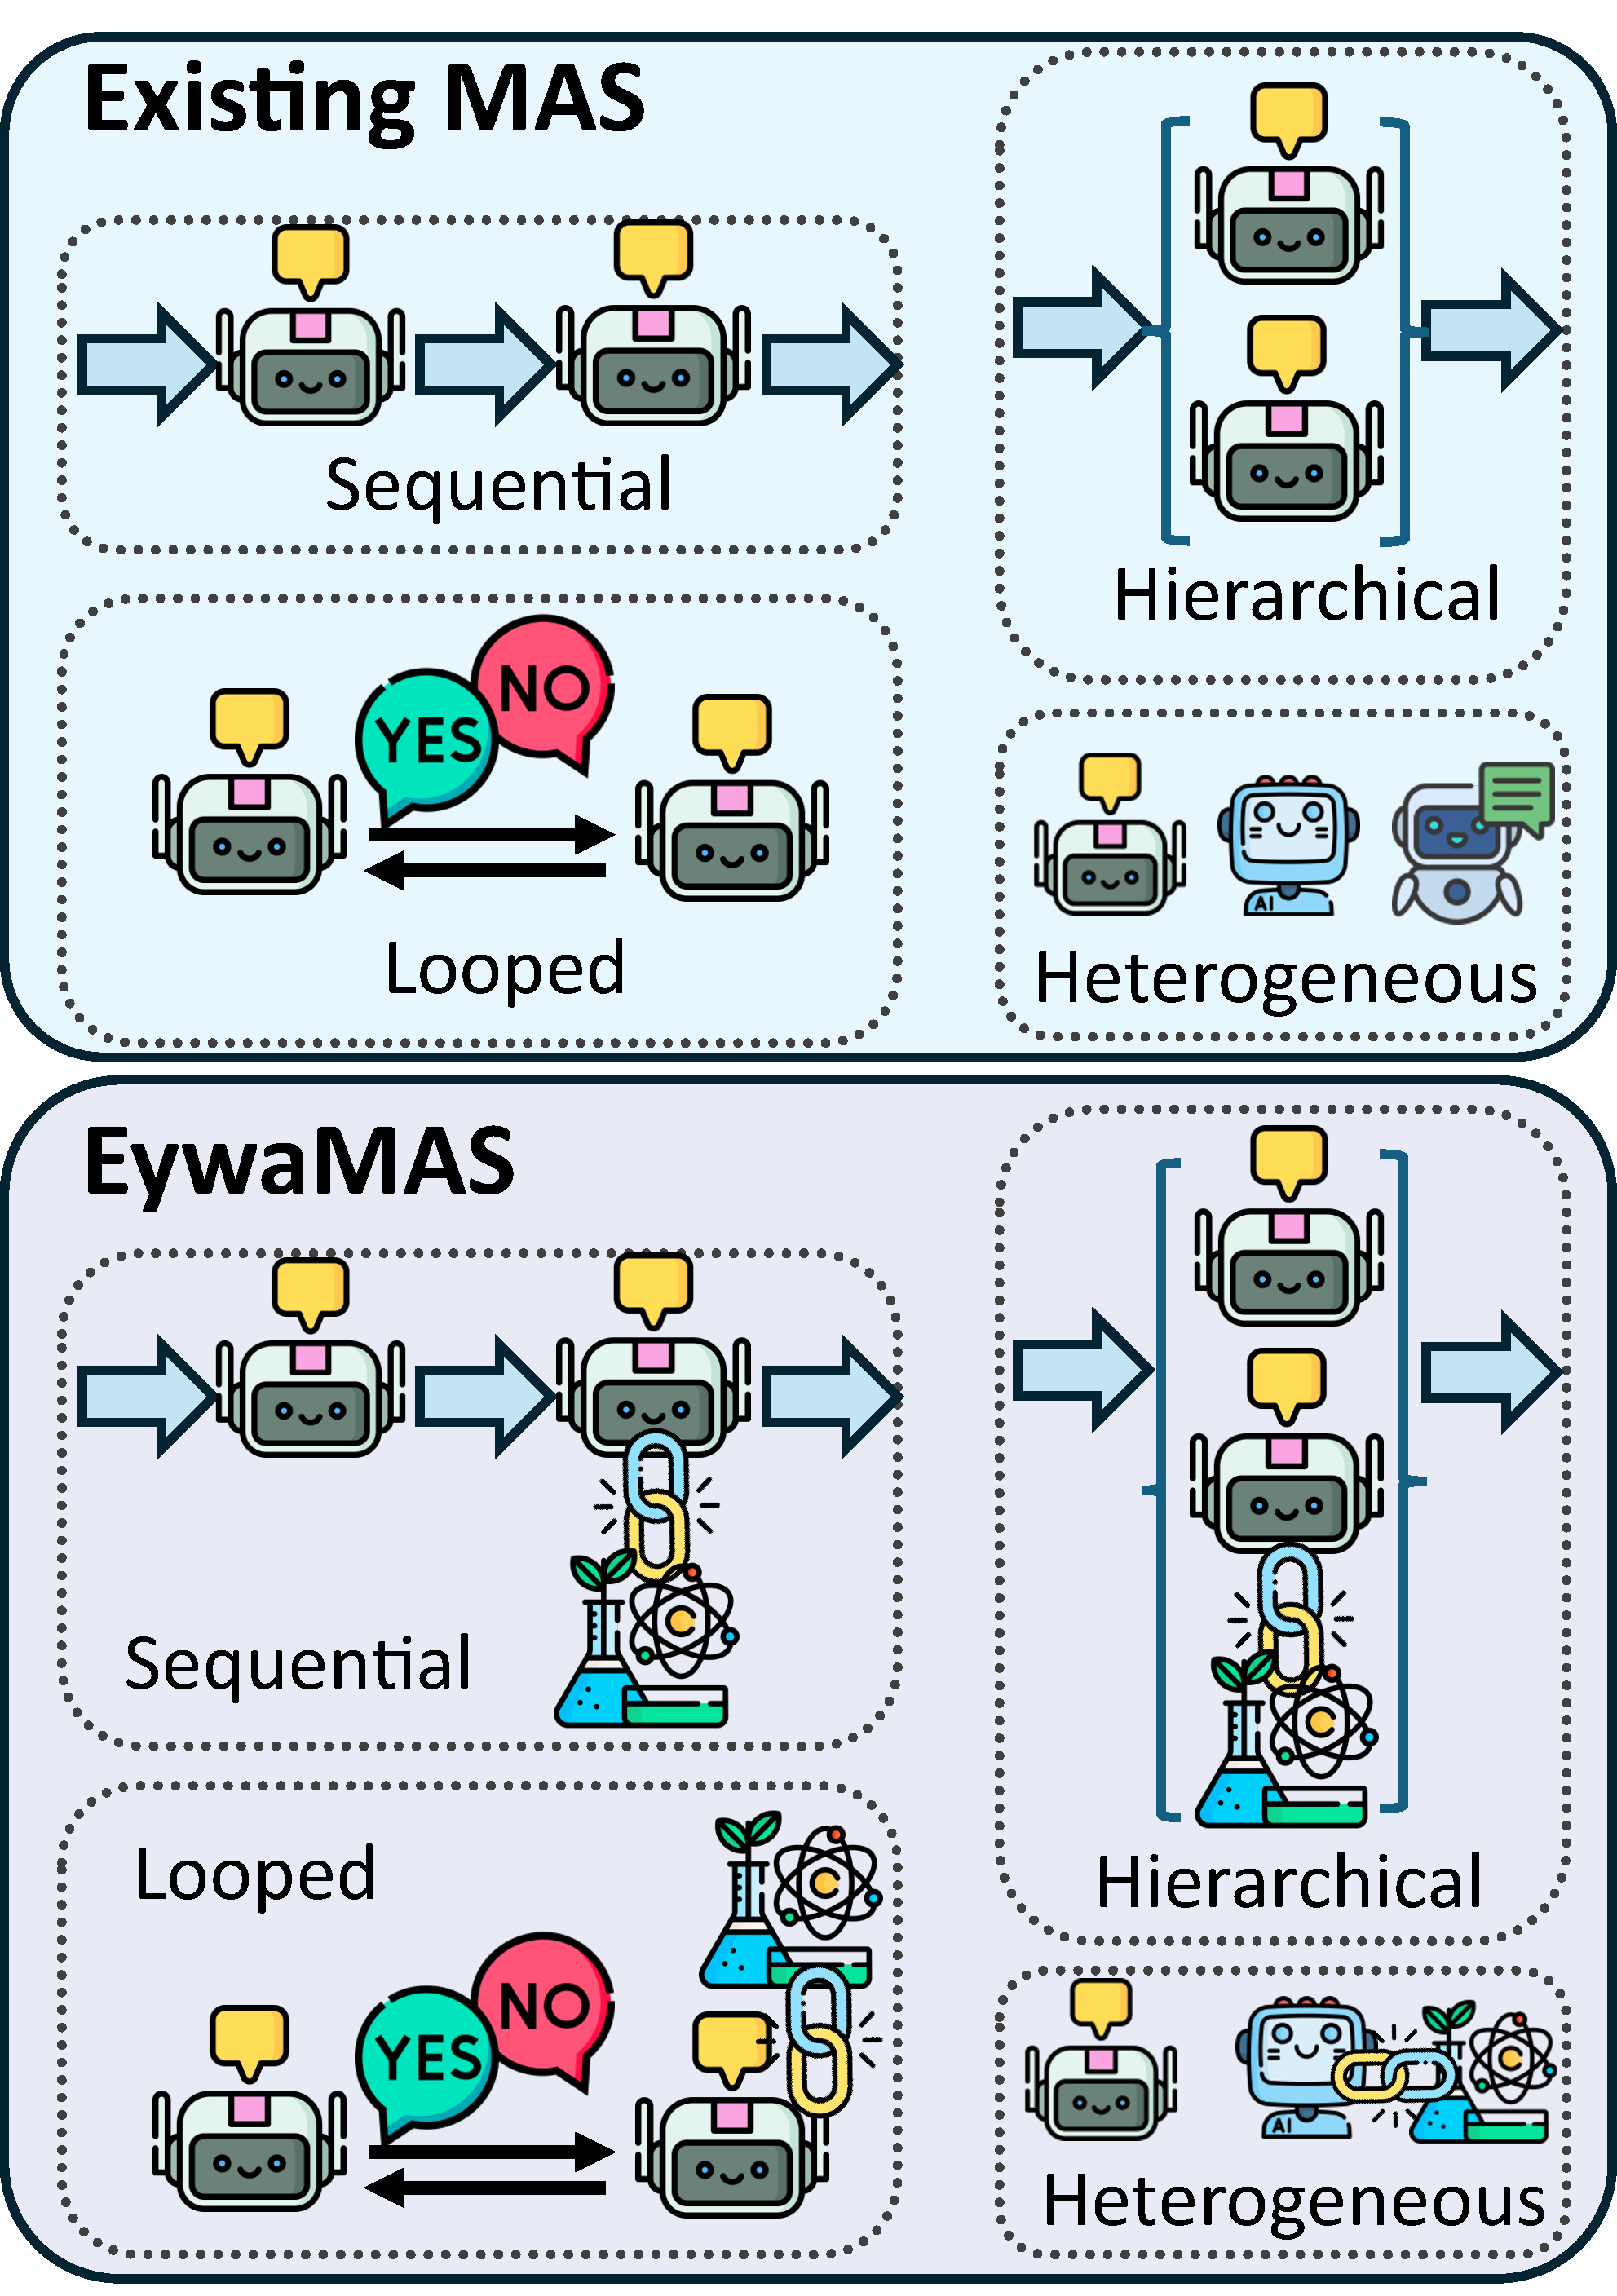
\includegraphics[width=0.30\textwidth]{figures/eywamas.pdf}
  \end{center}
  \vspace{-15pt}
  \caption{EywaMAS generalizes existing multi-agent systems with EywaAgents.}
  \vspace{-10pt}
\end{wrapfigure}

\textit{EywaMAS} is a multi-agent system that composes heterogeneous agents in a plug-and-play manner. Unlike traditional multi-agent systems that rely solely on language-based agents, EywaMAS enables seamless integration of both language-only agents and EywaAgents within a unified framework. In practice, constructing an EywaMAS requires minimal modification to existing multi-agent architectures. Specifically, one can replace a subset of language-only agents with EywaAgents while keeping the overall system structure unchanged. For example, in a hierarchical multi-agent system consisting of a planner, multiple worker agents, and a summarizer, substituting some of the worker agents with EywaAgents directly yields an EywaMAS. This plug-and-play property allows domain-specific foundation models to be incorporated into existing agentic systems without redesigning communication protocols or system architectures.


Each EywaAgent $\mathcal{A}_k$ internally follows the mechanism defined in Section~\ref{sec:eywaagent}, operating in the language space while optionally invoking its associated foundation model through the Tsaheylu interface.
At the system level, EywaMAS follows the same communication and state update dynamics as standard multi-agent systems, with interactions governed by the communication topology $\mathcal{G}$. 
As a result, EywaMAS forms a heterogeneous agentic system that integrates language-based reasoning with specialized foundation model capabilities in a unified and modular framework. It supports flexible composition across (1) different language models with varying scales or capabilities, (2) different foundation models across domains, and (3) mixed agent types (LLM Agents and EywaAgents).
When $\mathcal{A} =\{\mathcal{A}_1, \dots, \mathcal{A}_n\}$ are all LLM agents, EywaMAS degenerates to existing multi-agent systems. Similar to Theorem~\ref{thm:eywaagent improvement}, we establish a theoretical result showing that EywaMAS strictly improves over language-only multi-agent systems in Appendix \ref{app:mas}.


Compared to single-agent settings, EywaMAS enables parallel specialization and cross-domain collaboration. However, as communication topology is fixed and coordination is decentralized, the system may suffer from suboptimal topology or human configuration inefficiency, motivating the need for automatic orchestration.


\subsection{EywaOrchestra: Dynamic Orchestration of Heterogeneous Experts}

Real-world agentic tasks are highly diverse, and the optimal multi-agent organization for one task may be suboptimal for another. In particular, different tasks may require different mixtures of language-only reasoning, domain-grounded prediction, and inter-agent collaboration patterns. To address this, we extend \textit{Eywa} from static heterogeneous agents and fixed multi-agent systems to a dynamic orchestration framework, termed \textit{EywaOrchestra}.

\begin{tcolorbox}[
  agentscope,
  float,
  floatplacement=h,
  title=\textbf{EywaOrchestra}
]
\begin{definition}[EywaOrchestra]
\label{def:eywaorchestra}
Given candidate language models $\mathcal{M}_{\mathrm{LLM}}$, candidate domain-specific foundation models $\mathcal{M}_{\mathrm{FM}}$, and a topology pool $\Pi$, \textit{EywaOrchestra} is a dynamically instantiated heterogeneous multi-agent system:
\begin{equation}
\mathcal{O} = (\mathcal{C}, P)
\end{equation}
where $\mathcal{C}$ is the configuration space induced by $(\mathcal{M}_{\mathrm{LLM}}, \mathcal{M}_{\mathrm{FM}}, \Pi)$, $P$ is the conductor.
\end{definition}
\end{tcolorbox}

Planning in \textit{EywaOrchestra} is achieved by a \emph{conductor} that, conditioned on the input task, dynamically instantiates a heterogeneous multi-agent system by deciding: 
(i) the role and type of each agent, e.g., whether an agent should be a language-only agent or an EywaAgent;
(ii) the backbone language model used by each agent;
(iii) the domain-specific foundation model attached to each EywaAgent; and
(iv) the communication topology of the overall multi-agent system.
For tractability in this initial study, we assume a finite \emph{topology pool} of candidate multi-agent structures. In the current implementation, the \emph{conductor} is instantiated as a large language model that maps the input task to a system configuration from this pool. After the conductor selects a configuration, the instantiated system is executed to solve the task.


\begin{algorithm}[t]
\caption{EywaOrchestra: Dynamic Orchestration of Heterogeneous Experts}
\label{alg:eywaorchestra}
\begin{algorithmic}[1]
\REQUIRE Task input $\tau = (q, x, y^\star, \ell)$, configuration space $\mathcal{C}$, conductor $P$
\ENSURE Output $\hat{y}$

\STATE Select a system configuration $c \leftarrow P(q,x)$

\STATE Instantiate the heterogeneous agent system specified by $c$

\STATE Execute the induced multi-agent system on $(q,x)$ and return output $\hat{y}$
\end{algorithmic}
\end{algorithm}

The benefit of \textit{EywaOrchestra} can be understood through the gap between adaptive orchestration and any fixed configuration. Let $F_c$ denote the agent system instantiated by configuration $c$. Define the best fixed configuration risk as
\begin{equation}
\mathcal{R}_{\mathrm{fixed}}^\star
=
\min_{c\in\mathcal{C}}
\mathbb{E}_{\tau\sim\mathcal{T}}
\big[\ell(F_c(q,x),y^\star)\big],
\end{equation}
and the oracle adaptive risk as
\begin{equation}
\mathcal{R}_{\mathrm{oracle}}
=
\mathbb{E}_{\tau\sim\mathcal{T}}
\Big[
\min_{c\in\mathcal{C}}
\mathbb{E}\big[\ell(F_c(q,x),y^\star)\big]
\Big].
\end{equation}
By construction, $\mathcal{R}_{\mathrm{oracle}} \le \mathcal{R}_{\mathrm{fixed}}^\star$, with strict inequality whenever different regions of the task distribution favor different system configurations. This observation highlights the limitation of any fixed multi-agent design across various tasks. The motivation of \textit{EywaOrchestra} is precisely to move beyond such static designs by enabling task-adaptive system construction, jointly leveraging \emph{model adaptivity}, through selecting language and domain-specific foundation models, and \emph{structural adaptivity}, through selecting the communication topology itself.